\section{Utilization}
\label{sec-utilization}

\begin{table*}[t]
\centering
\caption{Typical LLM utilization methods and their key points for ICL, CoT, and planning. Note that the key points only highlight the most important technical contribution.} 
\label{tab:utilization}
\resizebox{\textwidth}{!}{%
\begin{tabular}{l|l|l}
\toprule
\textbf{Approach}                              & \textbf{Representative Work}     & \textbf{Key Point}                                                              \\
\midrule
\multirow{6}{*}{\begin{tabular}[c]{@{}l@{}}In-context\\Learning~(ICL)\end{tabular}} & KATE~\cite{Liu-ACL-2022-What}         & Demonstration selection (similar; k-NN)                      \\
                                                                                    & EPR~\cite{Rubin-NAACL-2022-Learning}  & Demonstration selection (dense retrieval; constrative learning)    \\
                                                                                    & SG-ICL~\cite{Kim-2022-arxiv-Self}     & Demonstration selection (LLM as the demonstration generator) \\
                                                                                    & APE~\cite{Zhou-2023-ICLR-Large}       & Demonstration format (automatic generation \& selection)                         \\
                                                                                    & Structured Prompting~\cite{Hao-2022-arxiv-Structured} & Demonstration format (grouped context encoding; rescaled attention) \\
                                                                                    & GlobalE \& LocalE~\cite{Lu-ACL-2022-Fantasically}     & Demonstration order (entropy-based metric; probing set generation with LLM) \\
\midrule
\multirow{6}{*}{\begin{tabular}[c]{@{}l@{}}Chain-of-thought\\Prompting~(CoT)\end{tabular}}  & Complex CoT~\cite{Fu-arxiv-2022-Complexity}                       & Demonstration (complexity-based selection)                          \\
                                                                                            & Auto-CoT~\cite{Zhang-arxiv-2022-Automatic}                        & Demonstration (automatic generation)                             \\
                                                                                            & Selection-Inference~\cite{Creswell-2022-arXiv-selection}          & Generation (alternate between selection and inference)                      \\
                                                                                            & Self-consistency~\cite{Wang-arxiv-2022-Self-Consistency}          & Generation (diverse paths; self-ensemble)             \\
                                                                                            & DIVERSE~\cite{Li-arxiv-2022-On}                                   & Generation (diverse paths); Verification (step-wise voting)           \\
                                                                                            & Rationale-augmented ensembles~\cite{Wang-arxiv-2022-Rationale}    & Generation (rationale sampling) \\
\midrule
\multirow{13}{*}{Planning}            & Least-to-most prompting~\cite{Zhou-arxiv-2022-Least} & Plan generation (text-based; problem decomposition)                                                  \\
                                     & DECOMP~\cite{Khot-2022-arXiv-Decomposed}             & Plan generation (text-based; problem decomposition) \\
                                     & PS~\cite{Wang-arXiv-2023-Plan}                       & Plan generation (text-based) \\
                                     & Faithful CoT~\cite{Lyu-arxiv-2023-Faithful}          & Plan generation (code-based) \\
                                     & PAL~\cite{Gao-arxiv-2022-PAL}                        & Plan generation (code-based; Python) \\
                                     & HuggingGPT~\cite{Shen-2023-arXiv-Hugginggpt}         & Plan generation (code-based; models from HuggingFace) \\
                                     & AdaPlanner~\cite{Sun-2023-arXiv-adaplanner}          & Plan refinement (skill memory) \\
                                     & TIP~\cite{Lu-2023-arXiv-multimodal}                  & Feedback acquisition (visual perception) \\
                                     & RAP~\cite{Hao-2023-arXiv-reasoning}                  & Feedback acquisition (LLM as the world model); Plan refinement (Monte Carlo Tree Search) \\
                                     & ChatCoT~\cite{Chen-2023-arXiv-chatcot}               & Feedback acquisition (tool); Plan refinement (conversation between LLM and tools) \\
                                     & ReAct~\cite{Yao-2022-arXiv-react}                    & Feedback acquisition (tool); Plan refinement (synergizing reasoning and acting)                                       \\
                                     & Reflexion~\cite{Shinn-2023-arXiv-Reflexion}          & Feedback acquisition (text-based self-reflection); Plan refinement (dynamic memory)                   \\
                                     & Tree of Thoughts~\cite{Yao-arxiv-2023-Tree}          & Feedback acquisition (vote comparison); Plan refinement (tree-based search)                                                       \\
\bottomrule
\end{tabular}%
}
\end{table*}

After pre-training or adaptation tuning, 
a major approach to using LLMs is to design suitable \textit{prompting} strategies for solving various tasks. {In existing literature, task-specific prompts can be effectively learned through manual creation and automatic optimization.} 
{A representative prompting method is \textit{in-context learning}~\cite{Brown-NeurIPS-2020-Language, Dong-arxiv-2023-A}, which formulates the task description and/or demonstrations in the form of natural language text.}
In addition, \textit{chain-of-thought prompting}~\cite{Wei-arxiv-2022-chain} can be employed to enhance in-context learning by involving a series of intermediate reasoning steps in prompts.
Furthermore, \textit{planning}~\cite{Zhou-arxiv-2022-Least} is proposed for solving complex tasks, which first breaks them down into smaller sub-tasks and then generates a plan of action to solve these sub-tasks one by one.
We summarize representative work for these prompting approaches in Table~\ref{tab:utilization}.
Next, we will elaborate on the details of the four techniques.

\subsection{Prompting}
As discussed in previous work~\cite{Liu-survey-2023-Pre-train}, prompting is the major approach to utilizing LLMs for solving various tasks. 
Since the quality of prompts will largely influence the  performance of LLMs in specific tasks, there have been a series of studies proposed to generate suitable task prompts through manual creation or automatic optimization, which will be introduced in this section.



\subsubsection{Prompt Creation}\label{subsec:promptdesign}
The process of manually creating a suitable prompt is also called \emph{prompt engineering}~\cite{Liu-arxiv-2022-Design,White-arxiv-2023-Prompt}. 
A well-designed prompt is very helpful to elicit the abilities of LLMs for accomplishing specific tasks.
In this part, we will first introduce the key components of prompts and discuss several principles for prompt design. Then, we evaluate ChatGPT with different prompts to show the results on several representative tasks. 
We are aware that there have been several existing papers~\cite{Santu-arxiv-2023-TELeR,White-arxiv-2023-Prompt} and websites~\cite{OpenAI-OpenAI-2023-PromptGuide,Contributors-AIShort-2023-AIShort,Contributors-Github-2023-Awesome} that present the suggestions and guidelines to design good prompts. 
As a comparison, we mainly aim to discuss the key factors (ingredients and principles) that are useful for prompt creation, and provide experimental results and analysis on popular tasks as the reference to the beginners. 


\paratitle{Key Ingredients.}
Typically, there are four key ingredients that {depict the functionality of a  prompt for eliciting the abilities of LLMs to complete the tasks}, including task description, input data, contextual information, and prompt  style. To have an intuitive understanding of our discussion, we also present three prompt examples for question answering, meta-review generation, and text-to-SQL    in Table~\ref{tab:prompt-examples}.


\textbullet~\emph{Task description.}
A task description is typically a specific instruction that LLMs are expected to follow. 
In general, one  should clearly describe the task goal  in natural language. 
For the tasks with special input or output format, detailed clarifications are often needed, and one can further utilize keywords to highlight the special settings for better guiding LLMs in task completion. 


\textbullet~\emph{Input data.} 
In common cases, it is straightforward to describe input data (\eg an instance to be responded by LLMs) in natural language. 
For special input data, such as knowledge graph and table, it is necessary to {apply an appropriate and convenient way} %
to make them readable for LLMs.  %
For structured data, linearization is commonly used to transform the original records (\eg knowledge triples) into sequences~\cite{Jiang-2023-arxiv-StructGPT} due to the simplicity.  
Further, the programming language (\eg executable code) has also been utilized to formulate the structured data,  %
{which can also support using external tools (\eg program executor) to produce the precise results~\cite{Beurer-arxiv-2023-Prompting,Lu-arxiv-2023-Chameleon}.
}



\textbullet~\emph{Contextual information.}
In addition to the task description and input data, contextual or background information is also essential for specific tasks. For example, retrieved documents are highly useful for open-domain question answering as supporting evidence. Both the quality of the retrieved documents and their relevance to the question have an impact on the generated answers~\cite{Ren-arxiv-2023-Investigating}. 
Thus, it needs to include such information in a proper prompt pattern or expression format.
Furthermore, in-context task exemplars are also helpful for eliciting LLMs to accomplish a complex task, which can better depict the task goal, {the special output formats, and the mapping relation between input and output.}

 
\textbullet~\emph{{Prompt} style.}
For different LLMs, it is important to design a suitable prompt style for eliciting their abilities to solve specific tasks. 
Overall, one should express the prompt as a clear question or detailed instruction that can be well understood and  answered. 
In some cases, it is also useful to add the {prefix or suffix} to better guide LLMs.
For example, using the prefix ``\emph{Let us think step by step}'' can help elicit LLMs perform step-by-step reasoning, and using the prefix ``\emph{You are an expert on this task (or in this domain)}'' can boost the performance of LLMs in some specific tasks. 
Further, 
for chat-based LLMs (\eg ChatGPT), instead of directly feeding a long or complex task prompt, it is suggested to decompose it into multiple prompts for the sub-tasks and then feed them into LLMs via a multi-turn conversation~\cite{Chen-2023-arXiv-chatcot}.


\paratitle{Design Principles.} Based on the key ingredients of prompts, we summarize several critical design principles that can help create more  effective prompts for solving various  tasks.

\textbullet~\emph{Expressing the task goal clearly.}  {Task descriptions should not be ambiguous or unclear, which likely lead to inaccurate or inappropriate responses.} This highlights the need for clear and unambiguous directives when utilizing these models~\cite{Ouyang-arxiv-2022-Training}. A clear and detailed description should contain various elements to explain a task, including task objective, input/output data (\eg ``\emph{Given a long document, I want you to generate a concise summary.}''),  and the response constraints (\eg ``\emph{the length of the summary cannot exceed 50.}''). By providing a well-clarified task description, LLMs can more effectively understand the target task and generate the desired output.

{
\textbullet~\emph{Decomposing into easy, detailed sub-tasks.} To solve complex tasks, it is important to decompose the difficult task into several more easier, detailed sub-tasks for helping LLMs accomplish the goal step by step, which is closely related to the planning technique in Section~\ref{subsec-planning}.
}
For example, following the suggestion~\cite{Santu-arxiv-2023-TELeR}, we can explicitly list the {sub-tasks in the form of multiple numbered items} (\eg ``\emph{Braid a coherent narrative by performing the following tasks: 1. ...; 2. ...; 3. ...}''). By decomposing a target task into sub-tasks, LLMs can focus on solving easier   sub-tasks and finally achieve more accurate results for complex tasks. 

\textbullet~\emph{Providing few-shot demonstrations.} As discussed in Section~\ref{subsec-icl},  LLMs can benefit from in-context learning for solving complex tasks, where the prompts contain a small number of task examples of the desired input-output pairs, \ie few-shot demonstrations. Few-shot demonstrations can help LLMs learn the semantic mapping between input and output without parameter tuning.
In practice, it is suggested that one should generate a few high-quality demonstrations for the target task, which would highly benefit the final task performance. 


\textbullet~\emph{Utilizing model-friendly format.} 
Since LLMs are pretrained on specially constructed datasets, there are some prompt formats that can make LLMs better understand the instruction. For example, as the OpenAI documentation suggests, we can use \texttt{\#\#\#} or \texttt{"""} as a stop symbol to separate the instruction and context, which can be better understood by LLMs. As a general guideline, most existing LLMs perform a task better in English, thus it is useful to employ English instructions to solve difficult tasks based on machine translation.


\paratitle{Useful Tips.}
In addition to the design principles, we also present a collection of  useful prompt tips based on existing work or our empirical experiences in Table~\ref{tab-tips}. 
Note that these tips are suggested in a general manner, it does not indicate that they are  the best prompts for the corresponding tasks.  
This part will be continuously updated with more guidelines or tips. We  welcome readers to contribute to this collection of  prompt tips.
We present the detailed procedure to contribute to the prompt tips, at the link: \url{https://github.com/RUCAIBox/LLMSurvey/tree/main/Prompts}. 

\begin{table*}[htb]
    \centering
    \caption{A collection of useful tips for designing prompts {that are collected from online notes~\cite{Santu-arxiv-2023-TELeR,White-arxiv-2023-Prompt,OpenAI-OpenAI-2023-PromptGuide,Contributors-AIShort-2023-AIShort} and experiences from our authors}, where we also show the related ingredients and principles (introduced in Section~\ref{subsec:promptdesign}). We abbreviate principles as Prin. and list the IDs of the related principles for each prompt.  {\textcircled{1}: expressing the task goal clearly; \textcircled{2}: decomposing into easy, detailed sub-tasks; \textcircled{3}: providing few-shot demonstrations; \textcircled{4}: utilizing model-friendly format.}}
    \label{tab-tips}
\scriptsize %
\begin{tabular}{cp{0.75\textwidth}c}
\toprule
\textbf{Ingredient} & \textbf{Collected Prompts} & \textbf{
Prin.}\\
\midrule
\multirow{4}{*}{\textbf{Task Description}}  & T1. Make your prompt \underline{\textbf{as detailed as possible}}, \eg ``\emph{Summarize the article into a short paragraph within 50 words. The major storyline and conclusion should be included, and the unimportant details can be omitted.}'' & \textcircled{1} \\
& T2. It is helpful to let the LLM know that it is \textbf{\underline{an expert with a prefixed prompt}}, \eg ``\emph{You are a sophisticated expert in the domain of compute science.}'' & \textcircled{1} \\ 
& T3. Tell the model \textbf{\underline{more what it should do}}, but not what it should not do. & \textcircled{1} \\
& T4. To avoid the LLM to generate too long output, you can just use the prompt: ``\emph{Question: {} Short Answer: {}}''. Besides, you can also use the following suffixes, ``\emph{in a or a few words}'', ``\emph{in one of two sentences}''. & \textcircled{1} \\
\midrule
\multirow{2}{*}{\textbf{Input Data}} & I1. For the question required factual knowledge, it is useful to first \underline{\textbf{retrieve relevant documents}} via the search engine, and then \underline{\textbf{concatenate them into the prompt}} as reference. & \textcircled{4}\\
& I2. To highlight some important parts in your prompt, please \underline{\textbf{use special marks}}, \eg \emph{quotation} ($""$) and \emph{line break} ($\backslash$n). You can also use both of them for emphasizing. & \textcircled{4} \\ 
\midrule
\multirow{4}{*}{\textbf{Contextual Information}}  & C1. For complex tasks, you can \textbf{\underline{clearly describe the required intermediate steps}} to accomplish it, \eg ``\emph{Please answer the question step by step as: Step 1 - Decompose the question into several sub-questions, $\cdots$}'' & \textcircled{2} \\
& C2. If you want LLMs to provide the score for a  text, it is necessary to provide a \textbf{\underline{detailed description about the}} \textbf{\underline{scoring standard}} with examples as reference. & \textcircled{1} \\
& C3. When LLMs generate text according to some context (\eg making recommendations according to purchase history), instructing them with \textbf{\underline{the explanation about the generated result}} conditioned on context is helpful to improve the quality of the generated text. & \textcircled{2} \\
& C4. An approach similar to \textbf{\underline{tree-of-thoughts}} but can be \textbf{\underline{done in one prompt}}: \eg \emph{Imagine three different experts are answering this question. All experts will write down one step of their thinking, then share it with the group of experts. Then all experts will go on to the next step, etc. If any expert realizes they're wrong at any point then they leave. The question is} & \textcircled{2} \\
\midrule
\multirow{9}{*}{\textbf{Demonstration}} & D1. \underline{\textbf{Well-formatted in-context exemplars}} are very useful, especially for producing the outputs with complex formats. & \textcircled{3} \\
& D2. For few-shot chain-of-thought prompting, you can also use the prompt ``\emph{Let's think step-by-step}'', and the few-shot examples should be \textbf{\underline{separated by ``$\backslash$n''}} instead of full stop. & \textcircled{1}\textcircled{3} \\
& D3. You can also \textbf{\underline{retrieve similar examples}} in context to supply the useful task-specific knowledge for LLMs. To retrieve more relevant examples, it is useful to \textbf{\underline{first obtain the answer}} of the question, and then concatenate it with the question for retrieval. & \textcircled{3}\textcircled{4} \\
& D4. The \textbf{\underline{diversity of the in-context exemplars}} within the prompt is also useful. If it is not easy to obtain diverse questions, you can also seek to keep the \textbf{\underline{diversity of the solutions}} for the questions. & \textcircled{3} \\
& D5. When using chat-based LLMs, you can \textbf{\underline{decompose in-context exemplars into multi-turn messages}}, to better match the human-chatbot conversation format. Similarly, you can also decompose the reasoning process of an exemplars into multi-turn conversation. & \textcircled{3} \\
& D6. \textbf{\underline{Complex and informative}} in-context exemplars can help LLMs answer complex questions. & \textcircled{3} \\
& D7. As a symbol sequence can typically be divided into multiple segments (\eg $i_1, i_2, i_3$ $\longrightarrow$ $i_1, i_2$ and $i_2, i_3$), the preceding ones can be used \textbf{\underline{as in-context exemplars}} to guide LLMs to predict the subsequent ones,  meanwhile providing  historical information. & \textcircled{2}\textcircled{3} \\ %
& D8. \textbf{\underline{Order matters}} for in-context exemplars and prompts components. For very long input data, the position of the question (first or last) may also affect the performance. & \textcircled{3} \\
& D9. If you can not obtain the in-context exemplars from existing datasets, an alternative way is to use the \textbf{\underline{zero-shot}} \textbf{\underline{generated ones}} from the LLM itself. & \textcircled{3} \\
\midrule
\multirow{8}{*}{\textbf{Other Designs}}  & O1. Let the \underline{\textbf{LLM check its outputs}} before draw the conclusion, \eg ``\emph{Check whether the above solution is correct or not.}'' & \textcircled{2} \\
& O2. If the LLM can not well solve the task, you can \textbf{\underline{seek help from external tools}} by prompting the LLM to manipulate them. In this way, the tools should be encapsulated into callable APIs with detailed description about their functions, to better guide the LLM to utilize the tools. & \textcircled{4} \\
& O3. The prompt should be \textbf{\underline{self-contained}}, and better not include pronouns (\eg it and they) in the context. & \textcircled{1} \\
& O4. When using LLMs for \textbf{\underline{comparing}} two or more examples, the order affects the performance a lot. & \textcircled{1} \\
& O5. Before the prompt, \textbf{\underline{assigning a role for the LLM}} is useful to help it better fulfill the following task instruction, \eg \emph{``I want you to act as a lawyer''}. & \textcircled{1}\\
& O6. OpenAI models can perform a task better in English than other languages. Thus, it is useful to first \textbf{\underline{translate the input into English}} and then feed it to LLMs. & \textcircled{4} \\
& O7. For multi-choice questions, it is useful to \textbf{\underline{constrain the output space}} of the LLM. You can use a more detailed explanation or just imposing constraints on the logits. & \textcircled{1} \\
& O8. For sorting based  tasks (\eg recommendation), instead of directly outputting the complete text of each item after sorting, one can  \textbf{\underline{assign indicators}} (\eg \emph{ABCD}) to the unsorted items and instruct the LLMs to directly output the sorted indicators. & \textcircled{1} \\
\bottomrule
\end{tabular}
\end{table*}
%

\paratitle{Empirical Analysis.}
We further conduct empirical studies to present the impact of prompts on task performance.
To conduct the experiments, we select a variety of tasks that span language generation, knowledge utilization, complex reasoning, structure data generation, and information retrieval. 
For each task, we manually write a prompt that follows general guidelines introduced above. Note that the tested prompts may not be the optimal for these tasks, since they mainly aim to help readers understand how to write an effective prompt for solving different tasks. 
Also, we add a simplified  prompt as the comparison for most tasks.  
Following the experimental settings in Section~\ref{sec-empirical}, we examine the  3-shot performance of ChatGPT on complex reasoning tasks (Colored Objects and GSM8k), and zero-shot performance on other tasks.
We report the experimental results in Table~\ref{tab-instructions}, where we also include the supervised  performance in existing papers as reference. 

$\bullet$ \emph{Carefully designed prompts can boost the zero-shot or few-shot performance of ChatGPT.} 
By comparing the results of using different prompts on the same task, we can see that using the carefully designed prompts  can achieve better performance than the simpler ones. 
{In the carefully designed prompts, we provide a more clearly expressed task description (\eg WMT and WikiFact), or use a model-friendly format (\eg GSM8k and OBQA). 
For example, for WikiFact task, the prompt with a more detailed task description leads to a performance increase  from 29.25 to 31.21.} 

$\bullet$ {\emph{More complex tasks can benefit more from careful prompt engineering on ChatGPT.}
In the WikiFact and Colored Objects tasks, the designed prompts have greatly improved the performance of ChatGPT, \ie from 23.61 to 28.47 on WikiFact and from 53.20 to 66.75 on Colored Objects.
It indicates the necessity of prompt engineering for LLMs to perform well on complex tasks, since these tasks typically have specific output formats or require background knowledge. 
Our example prompts  provide more detailed task description (\eg output format and task goal),  which can help ChatGPT better understand the complex task requirement  for fulfilling it.}

$\bullet$  {\emph{For mathematical reasoning tasks, it is more effective to design specific prompts based on the format of programming language.}
For GSM8k, the designed prompt employs code-formatted few-shot demonstrations to convert this mathematical reasoning task into code generation task, which can leverage the strong code synthesis ability of ChatGPT for solving mathematical problems. 
Further, with the help of an external program executor, we are able to obtain more precise results instead of using LLMs for arithmetic operation.
As we can see, the performance is boosted from 78.47 to 79.30 on GSM8k, indicating the usefulness of programming language in mathematical reasoning tasks.} %



$\bullet$ {\emph{In knowledge utilization and complex reasoning tasks, ChatGPT with proper prompts achieves comparable performance or even outperforms the supervised baselines methods.}
In knowledge utilization and  complex reasoning tasks, ChatGPT with proper zero-shot or few-shot prompts can achieve comparable performance or even outperform the supervised  methods, {\eg 31.21 (ChatGPT) \emph{v.s.} 34.20 (supervised baseline) on WikiFact.} 
Despite that, ChatGPT still performs worse than supervised baseline models on some specific tasks (\eg ARC and WikiFact), since these supervised models have been specially optimized with task-specific data.  
}


$\bullet$ \emph{Through suitable prompt engineering, LLMs can handle some non-traditional NLP tasks.}  
{With the help of specific prompts, ChatGPT can also accomplish non-traditional NLP tasks, \ie the general recommendation and conversational recommendation. 
A key point is that these tasks can be well expressed or described in natural language. }
However, the performance of ChatGPT is still far from the referenced performance in these tasks, as LLMs cannot directly fit these tasks, which require specific domain knowledge and task adaptation~\cite{Zhang-2023-arxiv-recommendation,Hou-2023-arxiv-large}.



\begin{table*}[ht]
	\footnotesize
	\centering
 \caption{Example instructions collected from \cite{Santu-arxiv-2023-TELeR,Chang-arxiv-2023-How}. The \colorbox{LightSkyBlue1}{blue} text denotes the task description, the \colorbox{tPink}{red} text denotes the contextual information, the \colorbox{tGreen}{green} text denotes the demonstrations, and the \colorbox{Khaki1}{gold} text denotes the prompt style.} 
	\label{tab:prompt-examples}
	\begin{tabular}{p\textwidth}
		\toprule
            \rowcolor{LightSkyBlue1}{\fontfamily{ppl}\selectfont Use the provided articles delimited by triple quotes to answer questions. If the answer cannot be found in the articles, write ``I could not find an answer.''} \\
            \specialrule{0em}{1pt}{1pt}
            \rowcolor{tGreen}
            \rowcolor{tPink}{\fontfamily{ppl}\selectfont \textbf{Articles:} ``````Joao Moutinho is a Portuguese footballer who last played as a central midfielder for Premier League club Wolverhampton Wanderers and the Portugal national team.'''''' } \\
            \specialrule{0em}{1pt}{1pt}
            \rowcolor{tGreen}{\fontfamily{ppl}\selectfont \textbf{Question:} Is the following sentence plausible?
'Joao Moutinho was out at third.' } \\
            \rowcolor{tGreen}{\fontfamily{ppl}\selectfont \textbf{Answer:} \colorbox{Khaki2}{Let's think step by step. Joao Moutinho is a soccer player. Being out at third is part of baseball, not soccer.} So the answer is No.} \\
            \rowcolor{tGreen}{\fontfamily{ppl}\selectfont ...} \\
            \rowcolor{tGreen}{\fontfamily{ppl}\selectfont $<$Demonstrations$>$} \\
            \\
            {\fontfamily{ppl}\selectfont \textbf{Articles:} $<$insert articles, each delimited by triple quotes$>$} \\
            {\fontfamily{ppl}\selectfont \textbf{Question:} $<$insert question$>$} \\
            {\fontfamily{ppl}\selectfont \textbf{Answer:}} \\
            
            \midrule[0.9pt]
            \midrule[0.9pt]
            
            \rowcolor{LightSkyBlue1}{\fontfamily{ppl}\selectfont Prepare a meta-review by answering the following questions from the reviewer comments (provided after the questions).} \\
            \specialrule{0em}{1pt}{1pt}
            \rowcolor{Khaki1}{\fontfamily{ppl}\selectfont 1. Based on the reviewer’s comments, what are the core contributions made by this manuscript?} \\
            \rowcolor{Khaki1}{\fontfamily{ppl}\selectfont 2. What are the common strengths of this work, as mentioned by multiple reviewers?} \\
            \rowcolor{Khaki1}{\fontfamily{ppl}\selectfont 3. What are the common weaknesses of this work, as highlighted by multiple reviewers?} \\
            \rowcolor{Khaki1}{\fontfamily{ppl}\selectfont 4. What suggestions would you provide for improving this paper?} \\
            \rowcolor{Khaki1}{\fontfamily{ppl}\selectfont 5. What are the missing references mentioned by the individual reviews?} \\
            \specialrule{0em}{1pt}{1pt}
            \rowcolor{tGreen}{\fontfamily{ppl}\selectfont \textbf{The review texts are below:}  $<$insert three comments $R_1$, $R_2$, $R_3$ from the reviewers$>$} \\
            \rowcolor{tGreen}{\fontfamily{ppl}\selectfont \textbf{Meta-review:} $<$insert meta-review$>$} \\
            \rowcolor{tGreen}{\fontfamily{ppl}\selectfont ...} \\
            \rowcolor{tGreen}{\fontfamily{ppl}\selectfont $<$Demonstrations$>$} \\
            \\
            {\fontfamily{ppl}\selectfont Provide justification for your response in detail by explaining why you made the choices you actually made. A good output should be coherent, highlight major strengths/issues mentioned by multiple reviewers, be less than 400 words in length, and finally, the response should be in English only.} \\ 
            \\
            {\fontfamily{ppl}\selectfont \textbf{The review texts are below:} $<$insert three comments $R_1$, $R_2$, $R_3$ from the reviewers$>$} \\
            {\fontfamily{ppl}\selectfont \textbf{Meta-review:} } \\

            \midrule[0.9pt]
            \midrule[0.9pt]

            \rowcolor{tPink}{\fontfamily{ppl}\selectfont CREATE TABLE Highschooler (} \\
            \rowcolor{tPink}{\fontfamily{ppl}\selectfont ID int primary key,} \\
            \rowcolor{tPink}{\fontfamily{ppl}\selectfont name text,} \\
            \rowcolor{tPink}{\fontfamily{ppl}\selectfont grade int} \\
            \rowcolor{tPink}{\fontfamily{ppl}\selectfont );} \\
            \rowcolor{tPink}{\fontfamily{ppl}\selectfont /*} \\
            \rowcolor{tPink}{\fontfamily{ppl}\selectfont 3 example rows:} \\
            \rowcolor{tPink}{\fontfamily{ppl}\selectfont SELECT * FROM Highschooler LIMIT 3;} \\
            \rowcolor{tPink}{\fontfamily{ppl}\selectfont ID \quad name \quad grade} \\
            \rowcolor{tPink}{\fontfamily{ppl}\selectfont 1234 \quad Janie \quad 8} \\
            \rowcolor{tPink}{\fontfamily{ppl}\selectfont 5678 \quad Mary \quad 8} \\
            \rowcolor{tPink}{\fontfamily{ppl}\selectfont 9012 \quad Mike \quad 9} \\
            \rowcolor{tPink}{\fontfamily{ppl}\selectfont */} \\
            \specialrule{0em}{1pt}{1pt}
            \rowcolor{LightSkyBlue1}{\fontfamily{ppl}\selectfont Using valid SQLite, answer the following questions for the tables provided above.} \\
            \specialrule{0em}{1pt}{1pt}
            \rowcolor{tGreen}{\fontfamily{ppl}\selectfont \textbf{Question:}  What is Kyle's id?} \\
            \rowcolor{tGreen}{\fontfamily{ppl}\selectfont \textbf{SQL:} SELECT ID FROM Highschooler WHERE name=``Kyle'';} \\
            \rowcolor{tGreen}{\fontfamily{ppl}\selectfont ...} \\
            \rowcolor{tGreen}{\fontfamily{ppl}\selectfont $<$Demonstrations$>$} \\
            \\
            {\fontfamily{ppl}\selectfont \textbf{Question:} $<$insert question$>$} \\
            {\fontfamily{ppl}\selectfont \textbf{SQL:} } \\
            
            \bottomrule
	\end{tabular}
\end{table*}



\subsubsection{Prompt Optimization} \label{sec:prompt_opt} 
{Although manually creating task prompts is more intuitive, it is time consuming and, more importantly, models are highly sensitive to the crafted prompts---improper prompts will lead to low task performance (as shown in Table~\ref{tab-instructions}). Therefore, a large body of studies propose automatic optimization approaches for discrete prompts and continuous prompts to achieve the optimal performance~\cite{shin-EMNLP-2020-autoprompt,Li-ACL-2021-prefix}. In this part, we will detail these studies from two perspectives, \ie discrete prompts and continuous prompts.}

\paratitle{Discrete Prompt Optimization.}  {Discrete prompt is typically composed of a sequence of natural language tokens. Despite that the form is simple and flexible, optimizing prompts in discrete space is a challenging problem due to the combinatorial huge search space. To automatically search effective prompts for downstream tasks, existing studies propose a wide spectrum of discrete prompt approaches, which are detailed as follows.}

$\bullet$  {\textit{Gradient-based approaches.} This kind of approaches aims to optimize the prompt search process by maximizing the output likelihood via gradient update~\cite{shin-EMNLP-2020-autoprompt,Wen-CoRR-2023-Hard,Gao-ACL-2021-Making,Zhou-CoRR-2023-InstructZero}.
As a representative work, Auto-Prompt~\cite{shin-EMNLP-2020-autoprompt} proposes a gradient-guided  method to greedily searches the optimal token for each position of the prompt,  leveraging the gradient approximated by the change in the log-likelihood when replacing a prompt token with another candidate token from vocabulary. However, such a search process can be extremely expensive since it needs to evaluate each candidate token for each position of the prompt, leading to a number of additional forward passes. Therefore, improved gradient method~\cite{Wen-CoRR-2023-Hard} has been proposed by transforming discrete tokens into continuous embeddings and computing the gradient on continuous space during  optimization.}

$\bullet$ {\textit{RL-based approaches.} 
Since discrete prompts are difficult to be learned through gradient back-propagation, a number of studies propose to formulate the discrete prompt optimization as a reinforcement learning (RL) problem and leverage RL algorithms for optimization~\cite{Deng-EMNLP-2022-RLPrompt,Zhang-ICLR-2023-TEMPERA}. For example, RLPrompt~\cite{Deng-EMNLP-2022-RLPrompt} {trains a policy network to generate desired prompts with multiple reward functions}. In this approach, several effective reward stabilization strategies are also proposed to enhance the RL training efficiency.  Compared to previous work that requires sufficient data for training, TEMPERA~\cite{Zhang-ICLR-2023-TEMPERA} proposes to directly generate prompts at test time {by utilizing a pre-trained RL agent to sequentially edit different parts of an manually-written initial prompt. 
}}

$\bullet$  {\textit{Edit-based approaches.} 
For the above methods, gradient-based and RL-based tuning can be extremely computationally demanding for ever larger models, and may not be feasible for API-based model calls (\eg ChatGPT). Therefore, another line of work aims to directly edit existing prompts based on the task performance. Specifically, GPS~\cite{Xu-EMNLP-2022-GPS} borrows an idea from the genetic algorithm and proposes a genetic prompt search method that utilizes a language model (\ie T5) to edit prompts by  taking the cloze task form. In addition to model based edit methods, human-defined  operations can be also employed for prompt editing~\cite{Prasad-EACL-2023-GrIPS}, including delete, swap, paraphrase, and addition. Based on these operations, they iteratively edit the prompts and greedily search for the best prompt guided by the model performance on a small pool of examples.}

$\bullet$  {\textit{LLM-based approaches.} Due to the exceptional capacities of LLMs, an increasing number of studies directly leverage LLMs as prompt generator~\cite{Zhou-ICLR-2023-Large,Pryzant-CoRR-2023-Automatic,Yang-CoRR-2023-Large}. Specifically, APE~\cite{Zhou-ICLR-2023-Large}  utilizes an LLM to generate initial prompts, then selects the best prompt with the highest accuracy, and finally improves the best candidate through an iterative Monte Carlo search method. Similarly, APO~\cite{Pryzant-CoRR-2023-Automatic} instructs the LLM to generate text feedback on how to refine an old prompt into new improved prompts. However, their search in the prompt space might be inefficient {without fully considering the whole refinement trace of previous prompts}, thus potentially leading to sub-optimal results. Therefore, another study~\cite{Yang-CoRR-2023-Large} incorporates the previous prompts with their scores to instruct LLMs for progressively generating better new prompts. However, these approaches still struggle in exploring the vast space of effective prompts. Inspired by human-like trial-and-error, prompt optimization is further formulated as a strategic planning problem~\cite{Wang-CoRR-2023-PromptAgent} and uses Monte Carlo tree search to navigate the vast prompt space.}


\paratitle{Continuous Prompt Optimization.} %
{Different from discrete prompts, continuous prompts consist of a set of continuous embeddings, which can be directly optimized through the gradient update based on the loss of downstream tasks. Note that continuous prompt optimization has been  mainly studied in PLMs, but draws limited attention in era of LLMs due to their massive magnitudes of parameters. We include the discussion of this part for content completeness. In prior work, most studies typically rely on supervised learning to train continuous prompts based on task data. Furthermore, in data-scarce scenarios, transfer learning methods can be employed to alleviate the lack of labeled data on target tasks. These two approaches are detailed below. 
}

$\bullet$ {\textit{Prompt learning  with sufficient data.} In this approach, most existing methods regard continuous prompts as trainable model parameters and then leverage supervised learning to optimize the continuous prompts by minimizing the cross-entropy loss based on sufficient downstream task data~\cite{Li-ACL-2021-prefix,Lester-ACL-2021-The,Tang-COLING-2022-Context,Liu-arXiv-2021-P-tuning}. As discussed in Section~\ref{sec-PEFT-methods}, prefix tuning~\cite{Li-ACL-2021-prefix} prepends a sequence of prefixes (\ie a set of trainable continuous vectors) to each Transformer layer in language models, while prompt tuning~\cite{Lester-ACL-2021-The} only incorporates trainable prompt vectors at the input layer. By fixing the large-scale parameters of LLMs and only tuning continuous prompt vector, this kind of approaches can be extremely parameter-efficient (Section~\ref{sec-PEFT}). However, these approaches are typically independent of the inputs, lacking sufficient consideration of input semantics. Therefore, the authors in \cite{Tang-COLING-2022-Context} propose context tuning, where the continuous prompts are derived based on the input text and learned through the downstream task losses.}


$\bullet$  {\textit{Prompt transferring  with scarce data.} Supervised learning approaches demand in sufficient training data to learn optimal continuous prompts, which may not work well in data-scarce domains and tasks. To address this problem, SPoT~\cite{Vu-ACL-2022-SPoT} proposes a prompt-based transfer learning approach, which first learns  %
{a single continuous prompt} for several representative source tasks and then uses this prompt to initialize the prompt for a target task.  {However, this approach leverages the same prompt for solving all instances of the target task. For a single task, even a well-learned prompt may not be suitable for all the data instances from a large population.} To address this issue, an improved method~\cite{Li-NAACL-2022-Learning} designs an adaptive attention mechanism during the prompt transfer process to derive the target prompts,  considering both task- and instance-level information.  %
{The prompt transfer paradigm can leverage the knowledge of data-sufficient source tasks encoded in source prompts for  solving  data-scarce target tasks.}
}
\subsection{In-Context Learning}
\label{subsec-icl}
As a special prompting form, in-context learning~(ICL) is first proposed along with GPT-3~\cite{Brown-NeurIPS-2020-Language}, which has become a typical approach to utilizing LLMs. 

\subsubsection{ICL Formulation}
\label{subsubsec-icl-formulation}

As stated in~\cite{Brown-NeurIPS-2020-Language}, ICL uses a formatted natural language prompt, consisting of the task description and/or a few task examples as demonstrations.
Figure~\ref{fig:utilization} presents an illustration of ICL.
First, starting with a task description, a few examples are selected from the task dataset as demonstrations.
Then, they are combined in a specific order to form natural language prompts with specially designed templates.
Finally, the test instance is appended to the demonstration as the input for LLMs to generate the output.
Based on task demonstrations, LLMs can recognize and perform a new task without explicit gradient update.

Formally, let $D_k = \{ f(x_1, y_1), \dots, f(x_k, y_k) \}$ represent a set of demonstrations with $k$ examples, where $f(x_k, y_k)$ is the prompt function that transforms the $k$-th task example into natural language prompts.
Given the task description $I$, demonstration $D_k$, and a new input query $x_{k+1}$, the prediction of the output $\hat{y}_{k+1}$ generated from LLMs can be formulated as follows\footnote{
When ICL was introduced in the GPT-3's paper~\cite{Brown-NeurIPS-2020-Language}, it was originally defined to be a combination of the task description and demonstration examples, wherein either component is dispensable. Following this definition, when a LLM is required to solve an unseen task by using only task descriptions, it can be also considered to perform ICL for task solving, whereas the ICL ability can be enhanced by instruction tuning.   
}: 
\begin{equation}\label{eq-ICL-prompting}
     \text{LLM} \big(I, \underbrace{ f(x_1, y_1), \dots, f(x_k, y_k)}_{\text{demonstrations}}, f(\underbrace{x_{k+1}}_{\text{input}}, \underbrace{\vphantom{\hat{y}_{k+1}} \_\_\_}_{\text{answer}}) \big) \rightarrow \hat{y}_{k+1}.
\end{equation}
where the actual answer $y_{k+1}$ is left as a blank to be predicted by the  LLM. %
Since the performance of ICL heavily relies on demonstrations, it is important to properly design them in the prompts. 
According to the construction process in Equation~\eqref{eq-ICL-prompting}, we focus on three major aspects of formatting demonstrations in the prompts, including how to select examples that make up demonstrations, format each example into the prompt with the function $f(\cdot)$, and arrange demonstrations in a reasonable order.  

{
A comprehensive review of ICL has been presented in the survey paper~\cite{Dong-arxiv-2023-A}, and we suggest the readers referring to it for a more general, detailed discussion on this topic. Compared with this survey, we specially focus on the discussion of applying ICL to LLMs in two major aspects, \ie demonstration design and the underlying mechanism of ICL. 
}
Also, ICL has a close connection with instruction tuning (discussed in Section~\ref{sec-instruction}) in that  
{both utilize natural language to format the task or instances}. 
However, instruction tuning needs to fine-tune LLMs for adaptation, while ICL only prompts LLMs for utilization.  
{Furthermore, instruction tuning can enhance the ICL ability of LLMs to perform target tasks, especially in the zero-shot setting (only using task descriptions)~\cite{Chung-arxiv-2022-Scaling}.  
}

\begin{figure*}[t]
    \centering
    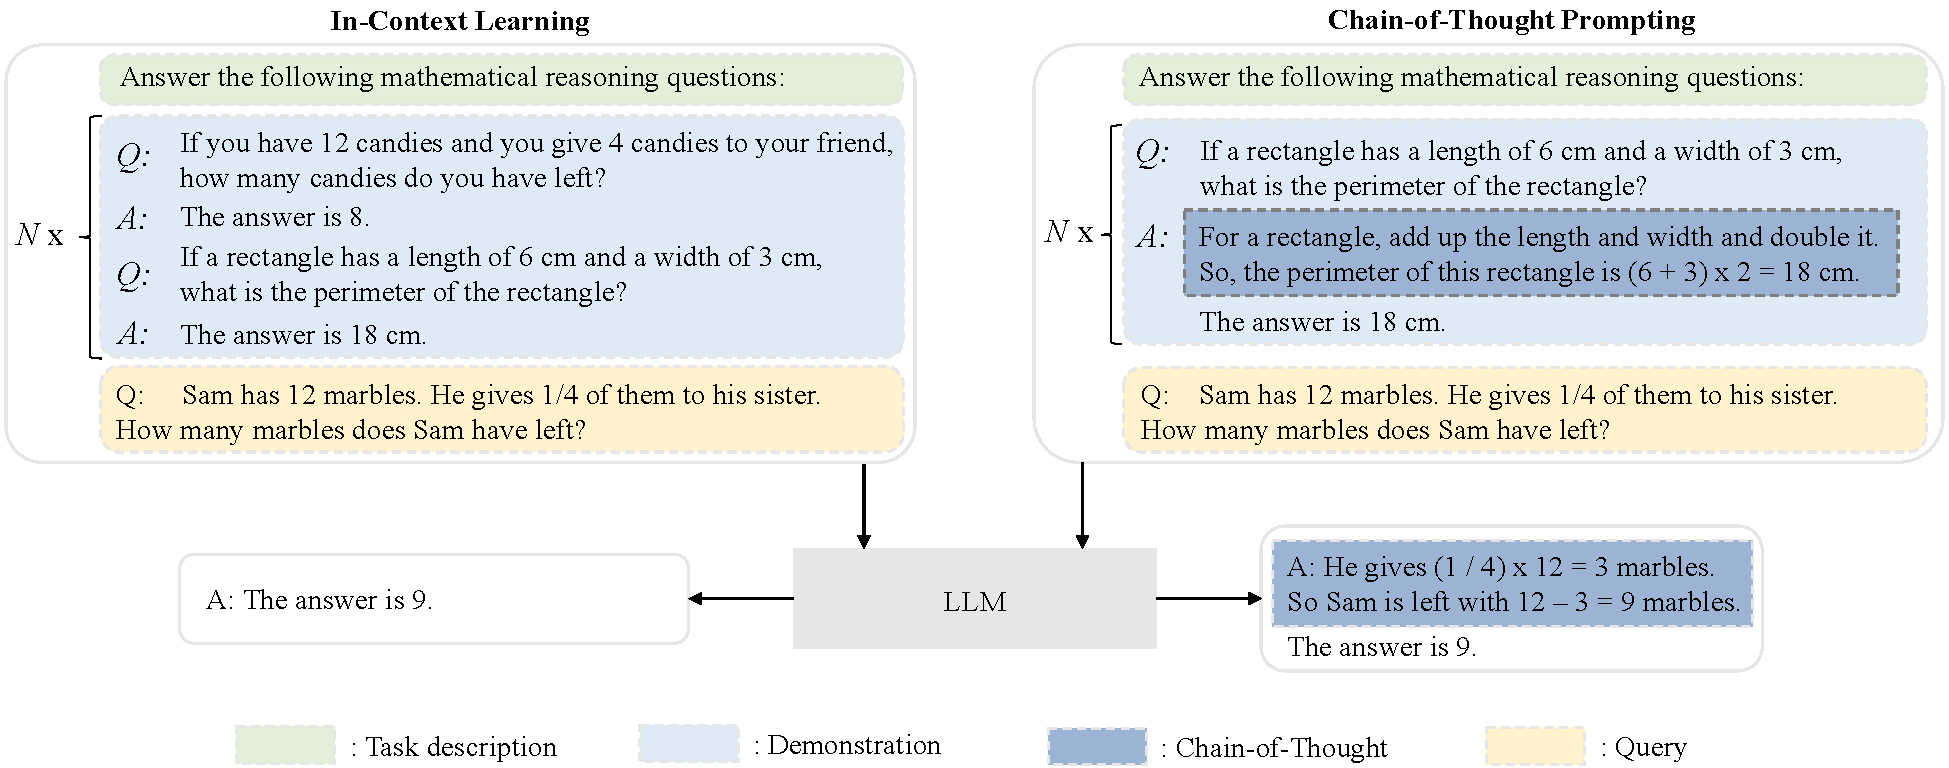
\includegraphics[width=\textwidth]{images/utilization.pdf}
    \caption{
        A comparative illustration of in-context learning~(ICL) and chain-of-thought~(CoT) prompting. 
        ICL prompts LLMs with a natural language description, several demonstrations, and a test query, while  
        CoT prompting involves a series of intermediate reasoning steps in prompts.
    }
    \label{fig:utilization}
\end{figure*}

\subsubsection{Demonstration Design}
{Several studies have shown that the effectiveness of ICL is highly affected by the design of demonstrations~\cite{Min-EMNLP-2022-Rethinking, Lu-ACL-2022-Fantasically,Zhao-ICML-2021-Calibrate}}
Following the discussion in {Section~\ref{subsubsec-icl-formulation}}, we will introduce the demonstration design of ICL from three major aspects, \ie demonstration selection, format, and order.

\paratitle{Demonstration Selection.}
{
The performance of ICL tends to have a large variance with different demonstration examples~\cite{Liu-ACL-2022-What}, so it is important to select a subset of examples that can effectively leverage the ICL capability of LLMs.}
There are two main demonstration selection approaches, namely heuristic and LLM-based approaches:


$\bullet$~\emph{Heuristic approaches.}  
{Due to their simplicity and low costs,} existing work widely adopts heuristic methods to select demonstrations.
Several studies employ a $k$-NN based retriever to select examples that are semantically relevant to the query~\cite{Liu-ACL-2022-What, Lee-COLING-2022-Does}.
{However, they perform the selection individually for each example, rather than evaluating the example set as a whole.}
To resolve this issue, diversity-based selection strategies are proposed to choose the most representative set of examples for specific tasks~\cite{Levy-arxiv-2022-Diverse, Su-arxiv-2022-selective}.
Furthermore, in~\cite{Ye-arxiv-2022-Complementary}, both relevance and diversity are taken into consideration when selecting demonstrations.


$\bullet$~\emph{LLM-based approaches.}  
Another line of work selects demonstrations by making use of LLMs. 
For example, LLMs can be utilized to directly measure the informativeness of each example according to the performance gain after adding the example~\cite{Li-arxiv-2023-Finding}. 
In addition, EPR~\cite{Rubin-NAACL-2022-Learning} proposes a two-stage retrieval approach that first recalls similar examples with an unsupervised method (\eg BM25) and then ranks them using a dense retriever (trained with positive and negative examples labeled by LLMs).
As an alternative approach, the task of demonstration selection can be formulated into a RL problem, where LLMs serve as the reward function to provide feedback for training the policy model~\cite{Zhang-EMNLP-2022-Active}. Since LLMs perform well for text annotation~\cite{Gilardi-arXiv-2023-Crowd}, some recent studies employ LLM itself as the demonstration generator without human intervention~\cite{Kim-arxiv-2022-Self-Generated}. 

{To summarize, as discussed in~\cite{Michael-ICLR-2022-An}, the selected demonstration examples in ICL should contain sufficient information about the task to solve as well as be relevant to the test query, for the above two selection approaches.} 

\paratitle{Demonstration Format.}
After selecting task examples, the next step is to integrate and format them into a natural language prompt for LLMs. 
A straightforward method is to instantiate a pre-defined template with the corresponding input-output pairs~\cite{Liu-survey-2023-Pre-train}.
To construct more informative templates, recent studies consider adding task descriptions~\cite{Chung-arxiv-2022-Scaling} or enhancing the reasoning capability of LLMs with chain-of-thought prompts~\cite{Wei-arxiv-2022-chain}.
For instance, in~\cite{Mishra-ACL-2022-Cross}, the authors collect a large-scale dataset with task descriptions written by humans.
After tuning with this dataset, the performance on seen tasks can be boosted, and LLMs can also generalize to unseen tasks to some extent.
To reduce the annotation costs, a semi-automated approach has been proposed in~\cite{Wang-arXiv-2022-Self} by employing a seed set consisting of human-written task descriptions to guide LLMs to generate task descriptions for new tasks. 
Since it is costly to manually annotate demonstration formats for different tasks, some work also studies how to automatically generate high-quality ones. 
As two representative methods, Auto-CoT~\cite{Zhang-arxiv-2022-Automatic} leverages LLMs with the zero-shot prompt ``\emph{Let’s think step by step}'' for generating intermediate reasoning steps, while least-to-most prompting~\cite{Zhou-arxiv-2022-Least} first queries LLMs to perform problem decomposition and then utilizes LLMs to sequentially solve sub-problems based on the intermediate answers to previously solved ones.  

\paratitle{Demonstration Order.}
LLMs are shown to sometimes suffer from the {recency} bias, \ie they are prone to repeat answers that are near the end of demonstrations~\cite{Zhao-ICML-2021-Calibrate}. 
Thus, it is important to arrange demonstrations (\ie task examples) in a reasonable order.
Early work proposes several heuristic methods to quickly find a good order.  
For example, demonstrations can be directly organized according to their similarity to the query in the embedding space~\cite{Liu-ACL-2022-What}: the more similar, the closer to the end.
In addition, global and local entropy metrics can be used to score different demonstration orders~\cite{Lu-ACL-2022-Fantasically}. 
To integrate more task information, some recent studies propose to minimize the  
{code length} required to compress and transmit task labels, which is inspired by information theory~\cite{Wu-arxiv-2022-Self}.
However, these methods need additional labeled data as the {validation set to evaluate the performance of specific demonstration orders}. 
To eliminate this need, the authors in~\cite{Lu-ACL-2022-Fantasically} propose to sample the validation data from the LLM itself. 

\subsubsection{Underlying Mechanism}
\label{sec-ICL-mechanism}
After pre-training, LLMs can exhibit intriguing ICL capability without being updated.  
In what follows, we discuss two key questions about the ICL ability of LLMs, \ie ``\emph{how does pre-training affect the ICL ability}'' and ``\emph{how do LLMs perform ICL during inference}''.

\paratitle{How Pre-Training Affects ICL?} 
ICL is first proposed in GPT-3~\cite{Brown-NeurIPS-2020-Language}, and it has been shown that the ICL ability becomes more significant with a larger model size.
Further, some studies reveal that small-scale PLMs can also demonstrate a strong ICL ability by continual pre-training~\cite{Gu-arXiv-2023-Pre} or fine-tuning~\cite{Min-NAACL-2022-MetaICL} on specially designed training tasks, which typically involve additional task examples in the input during the training process.
It suggests that the design of training tasks is an important influence factor on the ICL capability of LLMs. 
Besides training tasks, recent studies have also investigated the relationship between ICL and pre-training corpora~\cite{Michael-ICLR-2022-An, Hahn-2023-arXiv-a}.
For example, ICL can be theoretically explained as the product of pre-training on documents that exhibit long-range coherence~\cite{Michael-ICLR-2022-An}. 
{
Further, another study~\cite{Hahn-2023-arXiv-a} theoretically analyzes  that when scaling parameters and data, LLMs based on next-word prediction can emerge the ability of ICL by learning from the compositional structure (\eg how words and phrases are combined to form larger linguistic units like sentences) present in language data.  %
}

\paratitle{How LLMs Perform ICL?}
At the inference stage, researchers focus on analyzing how the ICL capability operates based on given demonstrations since no explicit learning or updating is involved.
According to the discussion in~\cite{Pan-2023-arXiv-what}, there are two main ways for LLMs to utilize demonstrations: task recognition and task learning.  

$\bullet$~\emph{Task recognition.}
{In the first way, LLMs recognize the task from demonstrations and utilize the prior knowledge obtained from pre-training to solve new test tasks. 
A Probably Approximately Correct~(PAC) framework~\cite{Wies-2023-arXiv-the} has been proposed to assess the learnability of ICL.
It assumes that there exists a latent variable representing the task in the pre-training data, and LLMs have been shown to be capable of capturing this variable from demonstrations, enabling them to recognize the task in ICL.
Also, the interpretation of ICL as task recognition is  supported by several empirical studies~\cite{Min-EMNLP-2022-Rethinking, Webson-2022-NAACL-do}.
For example, it has been observed that replacing the inputs or labels of demonstrations with random ones sampled from the input or label space does not seriously hurt the performance of LLMs, indicating that LLMs mainly recognize the target task from demonstrations instead of learning from them~\cite{Min-EMNLP-2022-Rethinking, Pan-2023-arXiv-what}.
Similarly, LLMs can exhibit decent performance even if the prompt template is irrelevant or misleading~\cite{Webson-2022-NAACL-do}.}

$\bullet$~\emph{Task learning.}
{In the second way, LLMs learn new tasks unseen in the pre-training stage only through demonstrations.
Specially, task learning is   analyzed mainly from the perspective of gradient descent and considered as implicit fine-tuning~\cite{Oswald-arxiv-2022-Transformers, Dai-arxiv-2022-Why}.}
Then, ICL can be explained as follows: by means of forward computation, LLMs generate meta-gradients with respect to demonstrations and implicitly perform gradient descent via the attention mechanism.
Experiments also show that certain attention heads in LLMs are capable of performing task-agnostic atomic operations~(\eg copying and prefix matching), which are closely related to the ICL ability~\cite{Olsson-arxiv-2022-In}.
Furthermore, some studies abstract ICL as an algorithm learning process~\cite{rek-arxiv-2022-what}. 
For example, the authors in~\cite{rek-arxiv-2022-what} find that LLMs essentially encode implicit models through their parameters during pre-training.
With the examples provided in ICL, LLMs can implement learning algorithms such as gradient descent or directly compute the closed-form solution to update these models during forward computation.
Under this explanation framework, it has been shown that LLMs can effectively learn simple linear functions and even some complex functions like decision trees with ICL~\cite{rek-arxiv-2022-what}.

As discussed in a recent study~\cite{Pan-2023-arXiv-what}, LLMs exhibit the abilities of both task recognition and task learning in ICL, but the two abilities seem to be possessed with different model scales.
As shown in the experiments~\cite{Pan-2023-arXiv-what}, the ability of task recognition is easier to obtain, and even a small LM with only 350M parameters can exhibit this ability, while task learning can only emerge for LLMs with at least 66B parameters.
Another study~\cite{Wei-arxiv-2023-Larger} also supports this finding with specially designed experiments.
They set up the tasks with flipped and semantically unrelated labels in the experiment, which require task learning when performing ICL.
The results suggest that small LMs tend to disregard the labels and mainly depend on their prior knowledge to accomplish the task, while LLMs have the ability to surpass their prior knowledge and acquire new knowledge from demonstrations, resulting in better outcomes. 
Furthermore, to improve the task learning ability, Meta-In-Context Learning~\cite{Forno-2023-arXiv-meta} proposes to include multiple related tasks instead of just a single one in the prompt.
In addition, Symbol Tuning~\cite{Wei-2023-arXiv-symbol} fine-tunes LLMs on demonstrations with semantically unrelated labels (\eg foo/bar instead of positive/negative for sentiment analysis), forcing LLMs to learn the task from demonstrations instead of relying on prior knowledge.
\begin{figure*}[t]
    \centering
    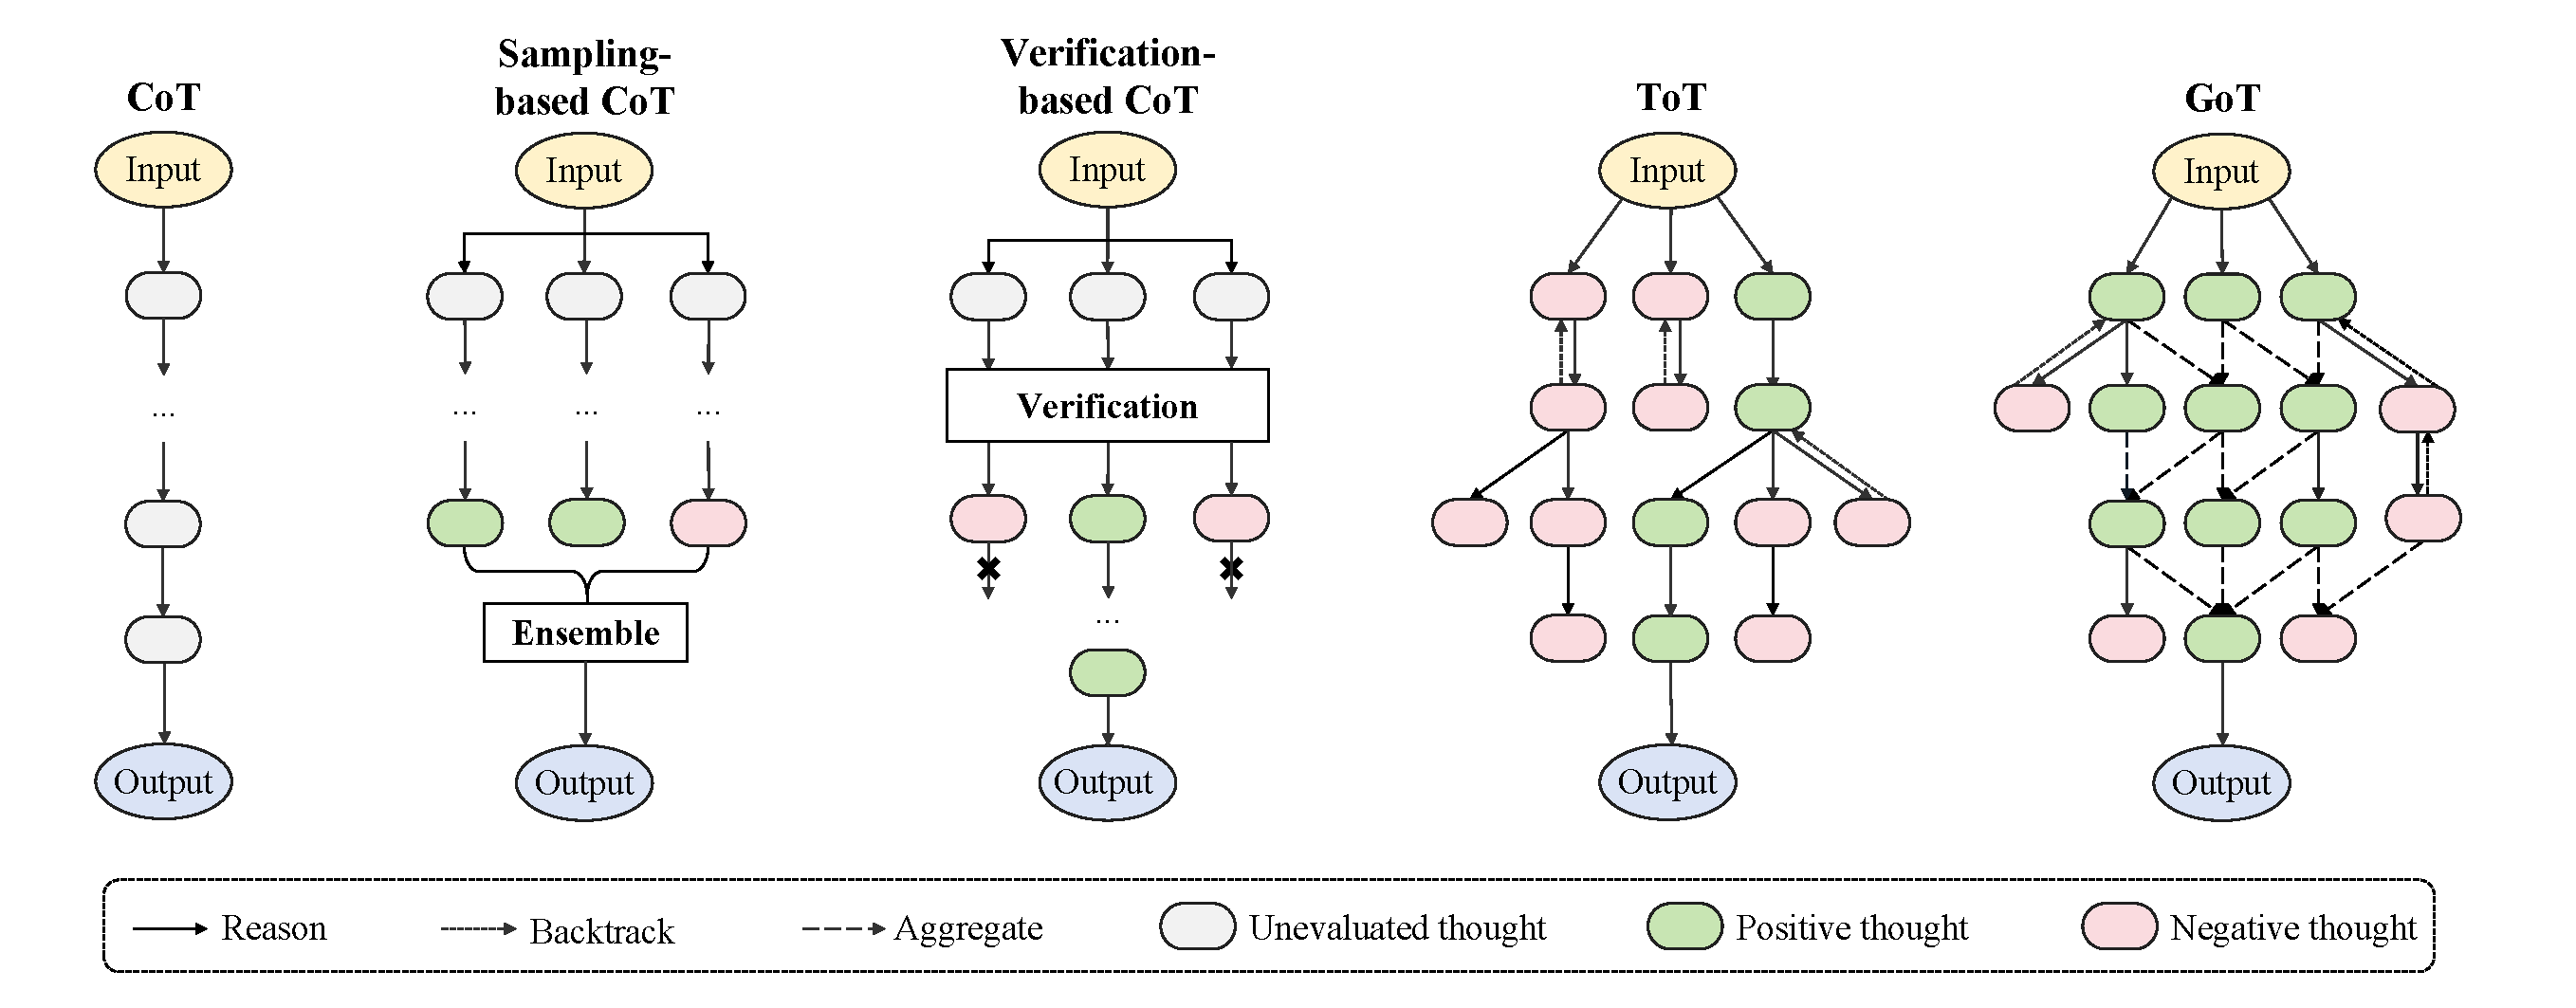
\includegraphics[width=\textwidth]{images/XoT.pdf}
    \caption{
        An illustration of the evolution of CoT prompting strategies. It begins with the basic CoT approach and progresses to enhanced CoT generation techniques,  including sampling-based and verification-based methods. Finally, it extends to variations of the chain structure, such as trees and graphs. Here, ``thought'' refers to an intermediate reasoning step as stated in~\cite{Wei-arxiv-2022-chain, Yao-arxiv-2023-Tree}.
    }
\label{fig:extension_of_CoT}
\end{figure*}

\subsection{Chain-of-Thought Prompting}
\label{subsec-cot}

Chain-of-Thought~(CoT) prompting~\cite{Wei-arxiv-2022-chain, Chu-arxiv-2023-A} is an improved prompting strategy to boost the performance of LLMs on complex reasoning tasks, such as arithmetic reasoning~\cite{Miao-ACL-2020-A}, commonsense reasoning~\cite{Talmor-naacl-2019-CommonsenseQA}, and symbolic reasoning~\cite{Wei-arxiv-2022-chain}.
Instead of simply constructing the prompts with input-output pairs like ICL, CoT prompting further incorporates intermediate reasoning steps, which serve as the bridge between inputs and outputs.
{
Figure~\ref{fig:utilization} presents an illustration of CoT.
In the following part, we will first elaborate on the basic CoT prompting approach and its improved strategies, then discuss when and why CoT prompting works.
}

\subsubsection{Basic CoT Prompting Approach}


{
}

CoT prompting is first proposed as an extension of ICL~\cite{Wei-arxiv-2022-chain}, which augments each demonstration $\langle$\emph{input, output}$\rangle$ as $\langle$\emph{input, CoT, output}$\rangle$.
A \textit{CoT} is a series of intermediate reasoning steps for connecting the \textit{input} and \textit{output}.
With these augmented demonstrations, LLMs can follow them to  %
{generate CoTs and the answer for a new input.} 
However, unlike $\langle$\emph{input, output}$\rangle$ pairs in ICL, CoTs are difficult to obtain and usually require human annotation.
Fortunately, it has been found that LLMs can be triggered to generate CoTs through simple instructions like ``\emph{Let's think step by step.}''~\cite{Kojima-arxiv-2022-Large}, making CoT prompting easy to use.
There are also alternative magic prompts that {can elicit the ability of CoT reasoning and further improve the performance of LLMs}, such as ``\emph{Take a deep breath and work on this problem step-by-step.}''~\cite{Yang-CoRR-2023-Large}.

{
As illustrated in Figure~\ref{fig:extension_of_CoT}, the generation process of CoT follows a chain structure in the basic CoT prompting approach, where LLMs generate CoTs step by step.
Typically, CoT takes the format of natural language text.
However, textual CoTs may not work well on complex tasks that require rigorous logic for reasoning.
Considering this, some work uses code~\cite{Chen-arxiv-2022-Program, Gao-ICML-2023-PAL} due to its structured and precise nature.
Furthermore, the authors in~\cite{Zhao-arxiv-2023-Automatic} propose to dynamically select text or code as the format of CoTs to combine their advantages.
}





\subsubsection{Improved CoT Prompting Strategies}

{
Despite the performance improvement in complex reasoning tasks, CoT prompting still suffers from problems like incorrect reasoning and instability.
In this part, we first introduce how to design better CoT prompts and enhanced CoT generation strategies, and then introduce the extension of the basic chain structure of CoT.
Figure~\ref{fig:extension_of_CoT} illustrates the evolution of representative CoT prompting strategies.
}

\paratitle{Better Prompt Design.}
Since CoT prompting relies on prompts to elicit the reasoning capabilities of LLMs, the design of prompts is critical to its performance.
As a direct approach, it is shown that using diverse CoTs (\ie multiple reasoning paths for each problem) can effectively enhance the performance~\cite{Li-arxiv-2022-On}.
Another intuitive idea is that prompts with more complex reasoning paths are more likely to elicit the reasoning ability of LLMs~\cite{Fu-arxiv-2022-Complexity}, which can result in higher accuracy in generating correct answers.
However, all these approaches rely on annotated CoT datasets, which limits their use in practice. 
To overcome this limitation, magic instructions such as  ``\emph{Let's think step by step}'' can be used to automatically construct CoTs by prompting LLMs~\cite{Zhang-arxiv-2022-Automatic}. 


\paratitle{Enhanced CoT Generation.}
{
Since LLMs are prone to producing incorrect reasoning steps and exhibiting instability in the generation process, there are a number of studies~\cite{Li-arxiv-2023-Making, Wang-arxiv-2022-Self-Consistency} to improve the generation of CoT.
In this part, we will introduce two typical approaches to enhancing the generation of CoT: sampling- and verification-based methods.
}

$\bullet$ \emph{Sampling-based methods.}
{
LLMs are known to suffer from instability during inference, which can lead to unfaithfulness in the generated reasoning steps.
To address this issue, some work proposes to sample multiple reasoning paths instead of using greedy decoding.
As a representative solution, self-consistency~\cite{Wang-arxiv-2022-Self-Consistency} 
first generates several reasoning paths and then takes an ensemble over the corresponding answers,  selecting the most consistent one through majority voting.
However, such a method can still lead to wrong answers when most of the reasoning paths are misled.
Considering this, the authors in~\cite{Fu-arxiv-2022-Complexity} only vote on the $k$ most complex reasoning paths based on their observation that reasoning paths with higher complexity (\eg more reasoning steps) usually have better performance. 
{Furthermore, MCR~\cite{Yoran-arxiv-2023-Answering} proposes referring to the steps from other reasoning paths when generating the next step, and performs reasoning across multiple reasoning paths to generate the final answer.}
}

$\bullet$ \emph{Verification-based methods.} {
The sequential nature of reasoning steps in CoTs can lead to the accumulation of errors in the generated CoTs when certain steps are incorrect. 
To mitigate this problem, recent studies propose to verify the correctness of generated reasoning steps with either trained verifiers or LLMs themselves. 
For example, DIVERSE~\cite{Li-arxiv-2023-Making} trains solution-level and step-level verifiers respectively to examine the reasoning steps at different granularities. 
Another approach~\cite{Ling-arxiv-2023-Deductive} utilizes LLMs to verify the correctness of reasoning steps through step-by-step self-verification with a specially designed reasoning format.
In addition, several studies propose backward reasoning for verification: 
it first deduces the necessary question conditions~\cite{Xue-arxiv-2023-RCOT, Weng-arxiv-2023-Large} or variables~\cite{Jiang-arxiv-2023-Forward} {from the model's predictions}, and then compares them with the original ones.
}

\paratitle{Reasoning Structure Extension.}   
{
Despite the generality, the chain reasoning structure of basic CoT prompting limits its effectiveness in solving complex tasks, which require exploration like foresight and backtracking during inference.
Therefore, many studies have been devoted to extending the reasoning structure by designing more intricate thought processes, \eg tree- and graph-structured reasoning. %
}

$\bullet$ \emph{Tree-structured reasoning.} 
This approach (exemplified by Tree of Thoughts~(ToT)~\cite{Yao-arxiv-2023-Tree, Long-arxiv-2023-Large}) formulates the reasoning process in a hierarchical tree structure, where intermediate thoughts are nodes.
{In this way, it enables  LLMs to explore multiple reasoning paths in parallel and further supports the operation of lookahead and backtracking to facilitate more comprehensive decisions.} 
In addition, TouT~\cite{Mo-arxiv-2023-Tree} takes the uncertainty of intermediate thoughts into account for thought evaluation based on Monte Carlo Dropout.

$\bullet$ \emph{Graph-structured reasoning.} {
Although the tree structure facilitates parallel reasoning, it also imposes restrictions on the reasoning process.
With more complex topological structures, graphs offer greater flexibility in reasoning, enabling the characterization of more intricate relationships and interactions.
For instance, Graph of Thoughts~(GoT)~\cite{Besta-arxiv-2023-Graph, Lei-arxiv-2023-Boosting} conceptualizes the reasoning process as an arbitrary graph, where vertices denote intermediate thoughts and edges denote the interdependence between these thoughts. 
{Compared with ToT, it can further utilize thoughts from other reasoning paths when generating new thoughts.}
However, such an approach requires a large number of interactions with LLMs, making the thought exploration process highly inefficient. 
} 
{
To reduce potentially meaningless thought exploration, XoT~\cite{ding-arxiv-2023-everything} further proposes to guide the search of thoughts with pre-trained policy and value networks.
}





\subsubsection{Further Discussion on CoT Prompting}
In this part, we present discussions regarding two fundamental questions related to CoT prompting, \ie ``\textit{when does CoT prompting work for LLMs}'' and ``\textit{why can LLMs perform CoT reasoning}''.

\paratitle{{When CoT Prompting Works For LLMs?}} 
Since CoT reasoning is an emergent ability~\cite{Wei-arxiv-2022-Emergent}, it only has a positive effect on sufficiently large models (typically containing 10B or more parameters~\cite{Wei-arxiv-2022-chain}) but not on small models. 
Moreover, since CoT prompting augments the standard prompting with intermediate reasoning steps, it is mainly effective for the tasks that require step-by-step reasoning~\cite{Wei-arxiv-2022-chain}, \eg arithmetic reasoning, commonsense reasoning, and symbolic reasoning.
Whereas, for other tasks that do not rely on complex reasoning, CoT prompting might lead to worse performance than standard prompting~\cite{Wang-arxiv-2022-Rationale}, \eg MNLI-m/mm, SST-2, and QQP from GLUE~\cite{Wang-EMNLP-2018-GLUE}.   
Interestingly, it seems that the performance gain brought by CoT prompting could be significant only when standard prompting yields poor results~\cite{Wei-arxiv-2022-chain}.

\paratitle{{Why LLMs Can Perform CoT Reasoning?}} 
As the second question, we discuss the underlying mechanism of CoT prompting in the following two aspects. 

$\bullet$ \emph{The source of CoT reasoning ability}. 
Regarding the source of CoT reasoning capability, it is widely hypothesized that it can be attributed to training on code since models trained on it show a strong reasoning ability~\cite{Liang-arxiv-2022-Holistic, FU-blog-2022-how, Bi-arxiv-2023-When}.   
Intuitively, code data is well organized with algorithmic logic and programming flow, which may be useful to improve the reasoning performance of LLMs. 
However, this hypothesis still lacks publicly reported evidence of ablation experiments (\emph{with} and \emph{without} training on code). 
In addition, instruction tuning seems not to be the key reason for obtaining the CoT reasoning ability, since 
it has been empirically shown that instruction tuning on non-CoT data does not improve the performance on held-out CoT reasoning benchmarks~\cite{Chung-arxiv-2022-Scaling}.

$\bullet$ \emph{The effect of CoT prompting components}. 
The major distinction between CoT prompting and standard prompting is the incorporation of reasoning paths prior to the final answer. 
Thus, some researchers investigate the effects of different components in the reasoning paths. 
Specifically, a recent study identifies three key components in CoT prompting, namely  \emph{symbols}~(\eg numerical quantities in arithmetic reasoning), \emph{patterns}~(\eg equations in arithmetic reasoning), and \emph{text}~(\ie the rest of tokens that are not symbols or patterns)~\cite{Madaan-arxiv-2022-Text}. 
It is shown that the latter two parts (\ie patterns and text) are essential to the model performance, and removing either one would lead to a significant performance drop. 
However, the correctness of symbols and patterns does not seem critical. 
Further, there exists a symbiotic relationship between text and patterns:   the text helps LLMs to generate useful patterns, and patterns aid LLMs to understand tasks and generate texts that help solve them~\cite{Madaan-arxiv-2022-Text}.


In summary, CoT prompting provides a general and flexible approach to eliciting the reasoning ability of LLMs. 
There are also some preliminary attempts to extend this technique to solve multimodal~\cite{Zhang-arxiv-2022-Multimodal} and multilingual tasks~\cite{Shi-arxiv-2022-Language}.
\subsection{Planning for Complex Task Solving}
\label{subsec-planning}
Prompting with ICL and CoT is a conceptually simple yet general approach to solving various tasks. 
However, this approach struggles with complex tasks like mathematical reasoning~\cite{Qian-2022-arXiv-limitations} and multi-hop question answering~\cite{Ning-arxiv-2023-ChatGPT}.
As an enhanced approach, prompt-based planning has been proposed to break down complex tasks into smaller sub-tasks and generate a plan of actions to accomplish the task.

\subsubsection{The Overall Framework}

\begin{figure}[t]
    \centering
    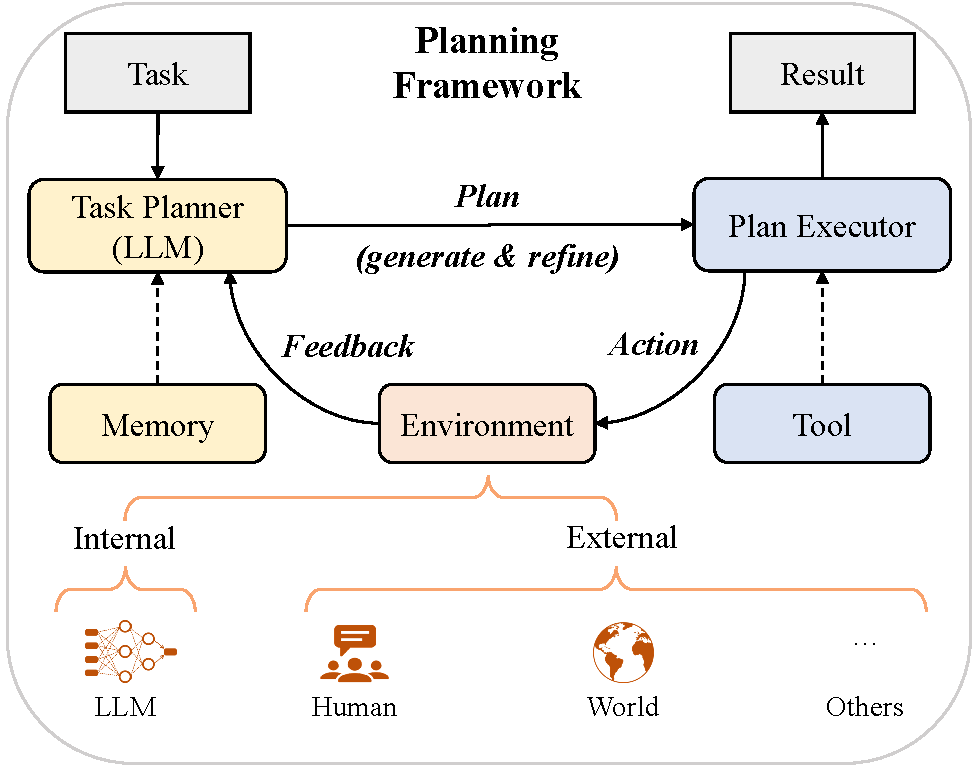
\includegraphics[width=\linewidth]{images/planning-v3.pdf}
    \caption{An illustration of the formulation for prompt based planning by LLMs for solving complex tasks.}
    \label{fig:planning}
\end{figure}

In this part, we first formulate the general planning paradigm of LLMs for solving complex tasks, which is illustrated in Figure~\ref{fig:planning}.

In this paradigm, there are typically three components: \emph{task planner}, \emph{plan executor}, and \emph{environment}\footnote{
Despite the similarity with RL, our formulation decouples the planning and execution phases, whereas in RL, they are typically interleaved in the agent.
This paradigm is defined in a general yet slightly loose way, and it mainly aims to help readers understand the key idea underlying the planning approaches of LLMs.
}.
Specifically, task planner, which is played by LLMs, aims to generate the whole plan to solve a target task.
The plan can be presented in various forms, \eg an action sequence in the form of natural language~\cite{Zhou-arxiv-2022-Least} or an executable program written in programming language~\cite{Gao-arxiv-2022-PAL}.
The LLM-based task planner can be enhanced with the memory mechanism for plan storage and retrieval, which is helpful for long-horizon tasks.
Then, plan executor is responsible for executing the actions in the plan.
It can be implemented by models like LLMs for textual tasks~\cite{Wang-arXiv-2023-Plan} or by tools like code interpreters for coding tasks~\cite{Shinn-2023-arXiv-Reflexion}.
Furthermore, environment refers to where the plan executor carries out the actions, which can be set differently according to specific tasks, \eg the LLM itself~\cite{Yao-2023-arXiv-tree} or an external virtual world like Minecraft~\cite{Wang-2023-arXiv-voyager}.
It provides \textit{feedback} about the execution result of the action to the task planner, either in the form of natural language~\cite{Shinn-2023-arXiv-Reflexion} or from other multimodal signals~\cite{Lu-2023-arXiv-multimodal}.

For solving a complex task, the task planner first needs to clearly understand the task goal and generate a reasonable plan based on the reasoning of LLMs (See Section~\ref{sec:plan-gen}).
Then, the plan executor acts according to the plan in the environment, and the environment will produce feedback for the task planner (See Section~\ref{sec:feedback}).
The task planner can further incorporate the feedback obtained from the environment to refine its initial plan and iteratively perform the above process to get better results as the task solution (See Section~\ref{sec:plan-refine}).


\subsubsection{Plan Generation}
\label{sec:plan-gen}
Plan generation focuses on directly generating action sequences by prompting LLMs.
Based on the format of the generated plans, existing work can be divided into two groups: text-based and code-based approaches. 

\paratitle{Text-based Approaches.}
It is straightforward for LLMs to generate plans in the form of natural language.
In this approach, LLMs are prompted to generate a sequence of actions for the plan executor to perform and solve the complex task.
For example, Plan-and-Solve~\cite{Wang-arXiv-2023-Plan} adds explicit instructions like ``\texttt{devise a plan}'' to directly prompt the LLM for planning in a zero-shot manner, while Self-planning~\cite{Jiang-arXiv-2023-Self} and DECOMP~\cite{Khot-2022-arXiv-Decomposed} add demonstrations in the prompt to guide the LLM to devise a plan through ICL.
Following this way, some work further considers incorporating extra tools or models when planning. 
For example, ToolFormer~\cite{Schick-arxiv-2023-Toolformer} first annotates a pre-training corpus with potential API calls using LLMs, and then fine-tunes LLMs on it,  so that LLMs can learn when and how to call APIs and incorporate the results returned by APIs during generation.
HuggingGPT~\cite{Shen-2023-arXiv-Hugginggpt} introduces the models available in HuggingFace and regards LLMs as the controller to select suitable models based on their descriptions and aggregate their results as the final solution.

\paratitle{Code-based Approaches.}
Although text-based approaches sound intuitive, they cannot guarantee faithful execution of the plan, which may lead to failure even when the plan is sound. 
To address this issue, code-based approaches have been proposed to generate more verifiable plans in the form of executable code in  programming languages, \eg Python or PDDL.
In this way, LLMs are first prompted to generate the program and then utilize a deterministic solver to execute it.
For example, Faithful CoT~\cite{Lyu-arxiv-2023-Faithful} and PAL~\cite{Gao-arxiv-2022-PAL} decompose a reasoning task into two stages: at the first stage, the LLM generates a plan conditioned on the query; at the second stage, a deterministic solver executes the plan to derive the final answer. 
Furthermore, code-based approaches can be applied to embodied agents in a similar way. 
For example, PROGPROMPT~\cite{Singh-arxiv-2022-ProgPrompt} and LLM+P~\cite{Liu-2023-arXiv-LLM+P} first utilize LLMs to generate plans in the form of python functions or PDDL files, and then leverage a virtual agent or classical planner to solve the problem according to the code-based plans.

\subsubsection{Feedback Acquisition}
\label{sec:feedback}
After executing the generated plan, the environment would produce the feedback signal to the LLM-based task planner, which can be used to refine its initial plan for better results.
In existing work, there are typically two sources of feedback from the environment, depending on their relationship with the LLM-based task planner: internal (\ie the LLM itself) and external (\eg tools or virtual worlds) feedback.

\paratitle{Internal Feedback.}
The LLM itself can be utilized as a feedback provider.
One straightforward way is to directly evaluate the quality of the generated plans through prompting.
For example, RAP~\cite{Hao-2023-arXiv-reasoning} evaluate the likelihood that each candidate plan can lead to task success, while Tree of Thoughts~\cite{Yao-2023-arXiv-tree} proposes to vote across plans by making comparisons between them.
Further, LLMs can provide feedback based on the intermediate results from the plan executor.
For example, Reflexion~\cite{Shinn-2023-arXiv-Reflexion} utilizes LLMs to transform sparse result signals (\eg success or failure) into concrete {text-based feedback (\eg ``\emph{You should recommend comedies that the user mentions in the query instead of horror movies}'') and stores this feedback in long-term memory for future planning.}


\paratitle{External Feedback.}
In addition to LLMs, external objects can also provide feedback signals.
For example, tools like code interpreters are widely used in programming tasks to provide real-time error messages~\cite{Shinn-2023-arXiv-Reflexion}, models like stable diffusion~\cite{Rombach-2022-CVPR-high} can be used in multimodal tasks to provide visual perception~\cite{Lu-2023-arXiv-multimodal}, and {virtual worlds} like Minecraft can provide immersive experiences~\cite{Wang-2023-arXiv-voyager}.
Besides, some work (\eg Generative Agents~\cite{Park-arxiv-2023-Generative}) explores multi-agent collaboration in simulated environments, where each agent receives feedback not only from interaction with the environment but also from communication with other agents.

\subsubsection{Plan Refinement}
\label{sec:plan-refine}
With access to feedback from the environment, the task planner can accordingly refine its current plan and iteratively go through the ``\emph{planning -- execution -- refinement}'' loop for better results.
In this part, we summarizes three major refinement approaches in existing work. 

\paratitle{Reasoning.}
The feedback data from the environment may not be directly suitable to be utilized by LLMs for plan refinement, \eg containing irrelevant information or taking a non-language form.
To solve this, some work adds the explicit reasoning process to extract critical information from feedback~\cite{Yao-2022-arXiv-react, Chen-2023-arXiv-chatcot}.
For example, React~\cite{Yao-2022-arXiv-react} prompts LLMs with demonstrations to generate reasoning traces over feedback.
It has been widely used in autonomous agent projects, such as AutoGPT~\cite{AutoGPT}, which can automatically reason over the observed feedback to revise the initial plan for solving various user requests.
However, these approaches typically fix the order of reasoning and planning.
To support flexible switching between the two processes for better performance, ChatCoT~\cite{Chen-2023-arXiv-chatcot} further unifies the tool-augmented reasoning process into a multi-turn conversation between the LLM-based task planner and the tool-based environment.

\paratitle{Backtracking.}
Early methods mainly consider planning forward actions while maintaining the existing plan, thus likely leading to local optimal plans based on a short-term evaluation.
To solve this, Tree of Thoughts~\cite{Yao-2023-arXiv-tree} allows backtracking with search algorithms like breadth-first and depth-first search to make global planning.
It refines the plan step by step by backtracking to the last state in the initial plan and choosing the next unexplored action.
Furthermore, some studies~\cite{Wang-2023-arXiv-describe, Lu-2023-arXiv-multimodal} utilize feedback signals to revise the entire plan.
For example, DEPS~\cite{Wang-2023-arXiv-describe} selects a better plan according to feedback signals, while TIP~\cite{Lu-2023-arXiv-multimodal} adds feedback signals to prompts for the LLM-based planner to revise each step in the initial plan.

\paratitle{Memorization.}
In order to handle long-horizon tasks, it has become a key approach to aid plan refinement with \emph{long-term memory} in addition to utilizing the \emph{short-term memory} of LLMs through ICL.
For example, Reflexion~\cite{Shinn-2023-arXiv-Reflexion} stores the feedback from self-reflection into the memory, so previous feedback can be retrieved for plan refinement.
Generative Agents~\cite{Park-arxiv-2023-Generative} designs the memory stream mechanism as the core component of agents for action planning and reflection.
Further, the skill library mechanism~\cite{Wang-2023-arXiv-voyager, Sun-2023-arXiv-adaplanner} is proposed to store successful plans in the library, which can be reused and synthesized as complex plans for novel tasks.
To implement the long-term memory mechanism, tools like vector databases (\eg milvus~\cite{Wang-2021-ICDM-Milvus}) can be used to encode plans or feedbacks into high-dimensional vectors for efficient storage and retrieval at a large scale.
MemoryBank~\cite{Zhong-2023-arxiv-MemoryBank} further proposes the memory updating mechanism to allow memory forgetting and strengthening following the Ebbinghaus Forgetting Curve theory.




